 \section{Evaluation}
 \label{sec:eval}

\Sys is developed in Python and leverages the PyTorch and Torch Geometric libraries to implement the federated graph learning framework. For developing the word2vec and vector harmonization module, we employ the Gensim library. Secure communication between clients and the utility server is ensured through Python's Cryptography module. All other functionalities of Sys are encapsulated in Python functions, designed for easy customization and deployment across different system environments.

We evaluate Sys using the open-source datasets Darpa E3 and OptC, which comprise system audit logs that simulate enterprise environments. These logs are collected from both Windows and Linux operating systems. Our evaluation experiments are conducted on a machine running Ubuntu 18.04.6 LTS, equipped with an 8-core Intel CPU and 100 GB of memory. Additionally, the machine features an NVIDIA RTX2080 GPU, utilized for operating our graph learning framework. Our evaluation aims to address the following research questions.

\begin{itemize}[leftmargin=*]
\item \textbf{Q1.} How does \Sys compares to existing systems in terms of detection performance?
\item \textbf{Q2.} What is the effectiveness of word2vec harmonization in a utility server setting?
\item \textbf{Q3.} What is the resource consumption of \Sys running on a client machine?
\item \textbf{Q4.} What is the end to end processing time of \Sys on a client machine?
\item \textbf{Q5.} What is the effect of varying differential privacy noise on detection performance?
\item \textbf{Q6.} Ablation study of various \Sys components.
\end{itemize}

\subsection*{Datasets}
\Sys underwent testing with two open-source datasets: \darpa E3~\cite{darpae3} and \darpa \optc~\cite{darpatc}. The E3 dataset, originating from \darpa's third red-vs-blue team exercise, includes audit logs depicting both normal and malicious activities. The \darpa \optc dataset offers a comprehensive view of benign and malevolent audit records from around 1000 hosts. It features six days of normal activities for training, followed by three days showcasing different types of attacks for evaluation purposes. The first day simulates a PowerShell Empire staging scenario, including the initial breach, lateral movements, and privilege escalations. The second day focuses on data exfiltration events, while the third day involves the deployment of malicious software.

\subsection*{Detectors for Comparison}

{\renewcommand{\arraystretch}{1.2}% for the vertical padding
\begin{table*}[t!]
  \centering
  \scriptsize
  \caption{Comparison of \Sys against FLASH and KAIROS. Prec.: Precision; Rec.: Recall;}
  \setlength{\tabcolsep}{0.7pt}
  \begin{tabular}{ccccccccccccc}
    \toprule

  \multirow{2}{*}{\textbf{Datasets}}
  & \multicolumn{4}{c }{\Norothead{ \bf \Sys}}
  & \multicolumn{4}{c }{\Norothead{ \bf FlASH}}
  & \multicolumn{4}{c }{\Norothead{ \bf KAIROS}}
  \\ \cmidrule(r{\tbspace}){2-5} \cmidrule(r{\tbspace}){6-9} \cmidrule(r{\tbspace}){10-13}

    & {\bf Prec.} &  {\bf Rec.} & {\bf \fscore} & {\bf TP}/ {\bf FP}/ {\bf FN}/ {\bf TN} & {\bf Prec.}  & {\bf Rec.} & {\bf \fscore} & {\bf TP}/ {\bf FP}/ {\bf FN}/ {\bf TN} & {\bf Prec.}  & {\bf Rec.} & {\bf \fscore} & {\bf TP}/ {\bf FP}/ {\bf FN}/ {\bf TN} \\

  \midrule

  E3-CADETS &  0.90 & 0.99 & 0.95 & 12846/ 1408/ 6/ 705,558 & 0.94 & 0.99 & 0.96 & 12851/ 818/ 1/ 706,148 & 0.80 & 1.00 & - & 4/ 1/ 0/ 174 \\
  E3-TRACE &  0.95 & 0.99 & 0.97 & 67357/ 3161/ 26/ 2,412,846 & 0.95 & 0.99 & 0.97 &  67382/ 3477/ 1/ 2,412,530 & - & - & - & - \\
  E3-THEIA &  0.89 & 0.99 & 0.94 & 25311/ 3155/ 51/ 3,502,171 & 0.92 & 0.99 & 0.95 & 25318/ 2282/ 44/ 3,503,044 & 0.67 & 1.00 & - & 10/ 1/ 0/ 216 \\  
  OpTC & 0.88 & 0.94 & 0.91 & 610/ 80/ 40/ 1,287,275 & 0.93 & 0.92 & 0.93 & 600/ 43/ 50/ 1,287,312 & 0.84 & 1.00 & - & 32/ 6/ 0/ 1210 \\
  \bottomrule
  \end{tabular}
\label{summary:benchmarks:large}
\end{table*}}

 \subsection*{Detection Performance}
 Table~\ref{summary:benchmarks:large} presents a comparative analysis of the detection performance between \Sys and \threatrace. It reveals that \Sys achieves a detection performance comparable to that of \threatrace. The advantage of \Sys lies in its ability to preserve user log privacy via federated learning. Additionally, its scalability is enhanced as each client independently conducts anomaly detection on their logs. This decentralization of learning and detection tasks, enabled by federated learning, significantly enhances the scalability of our system.

 \subsection*{Efficacy of Word2vec harmonization}
 To evaluate the efficacy of our method, we performed experiments comparing the utility server-based harmonized model with a local word2vec model on each client. These experiments utilized the \optc dataset. The findings, detailed in Table~\ref{local:wordvec}, demonstrate that our strategy significantly enhances the performance of \Sys. This improvement is attributed to our approach's ability to minimize noise in disparate word2vec vectors, thereby facilitating a more accurate interpretation of various activity patterns in the provenance graph by the \gnnshort model.

 \subsection*{CPU and Resource Consumption}

 \subsection*{Processing Time Analysis}

 \subsection*{Effect of Differential Privacy}

 \subsection*{Ablation Study}



\PP{Effect of Hosts vs Detection Performance}

\PP{Effect of Federated Learning Rounds}


\begin{table}[h!]
  \centering
  \scriptsize
    \caption{Effectiveness of word2vec vectors harmonization.}
      \begin{tabular}{ | c | c | c | c | c | c |}
        \hline
          \bf Word2vec Type & \bf Precision & \bf Recall & \bf \fscore & \bf TP & \bf FP \\
        \hline
         Vanilla & 0.66  & 0.97 & 0.79 & 636 & 325 \\
         Harmonized & 0.88 & 0.94 & 0.91 & 610 & 80 \\
        \hline
      \end{tabular}
      \label{local:wordvec}
  \end{table}

\begin{figure}[t!]
  \centering
  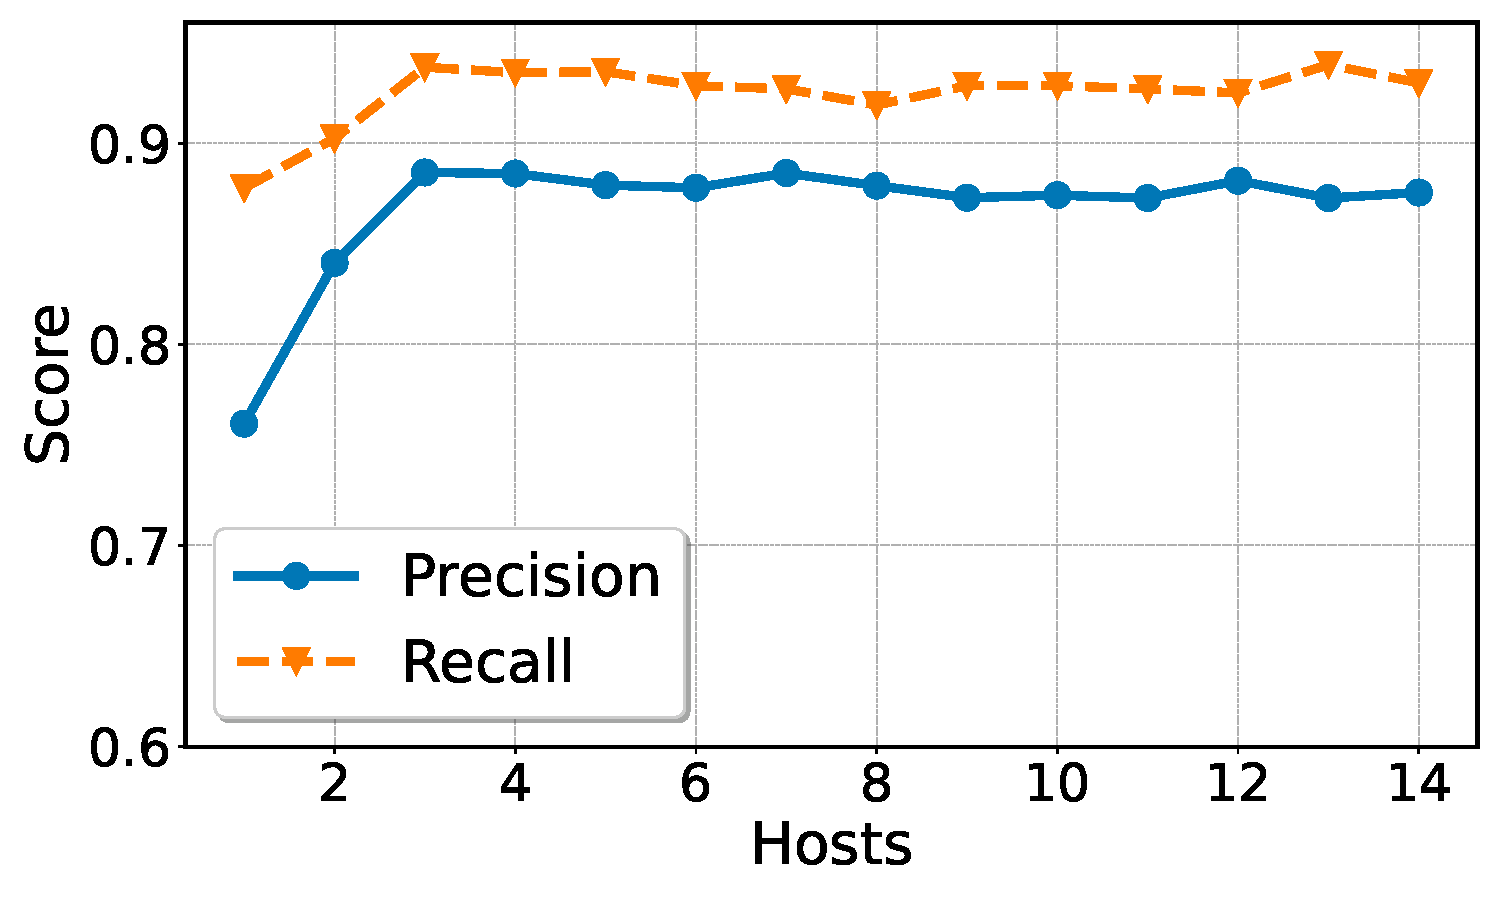
\includegraphics[width=0.50\textwidth]{fig/scoresvshosts.pdf}
  \caption{Effect of number of hosts vs detection metrics.}
  \label{scoresvshosts}
  \vspace{-2ex}
\end{figure}

\begin{figure}[t!]
  \centering
  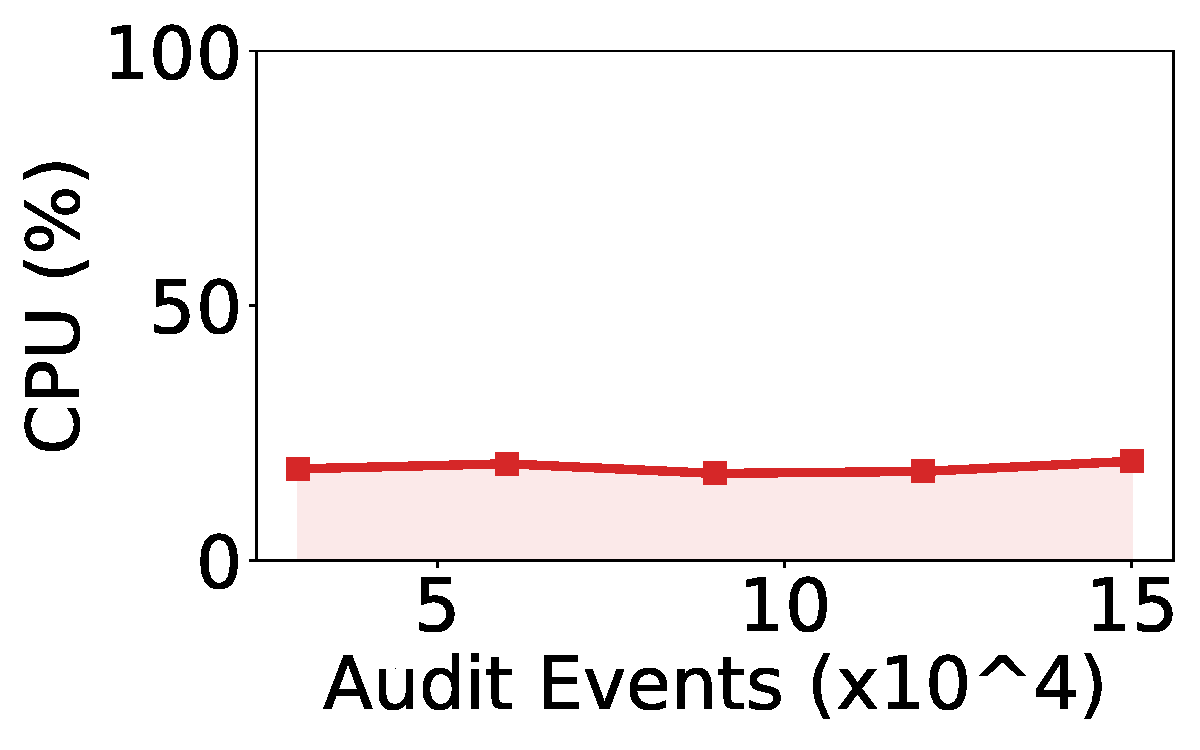
\includegraphics[width=0.50\textwidth]{fig/cpu.pdf}
  \caption{CPU Usage}
  \label{cpu}
  \vspace{-2ex}
\end{figure}

\begin{figure}[t!]
  \centering
  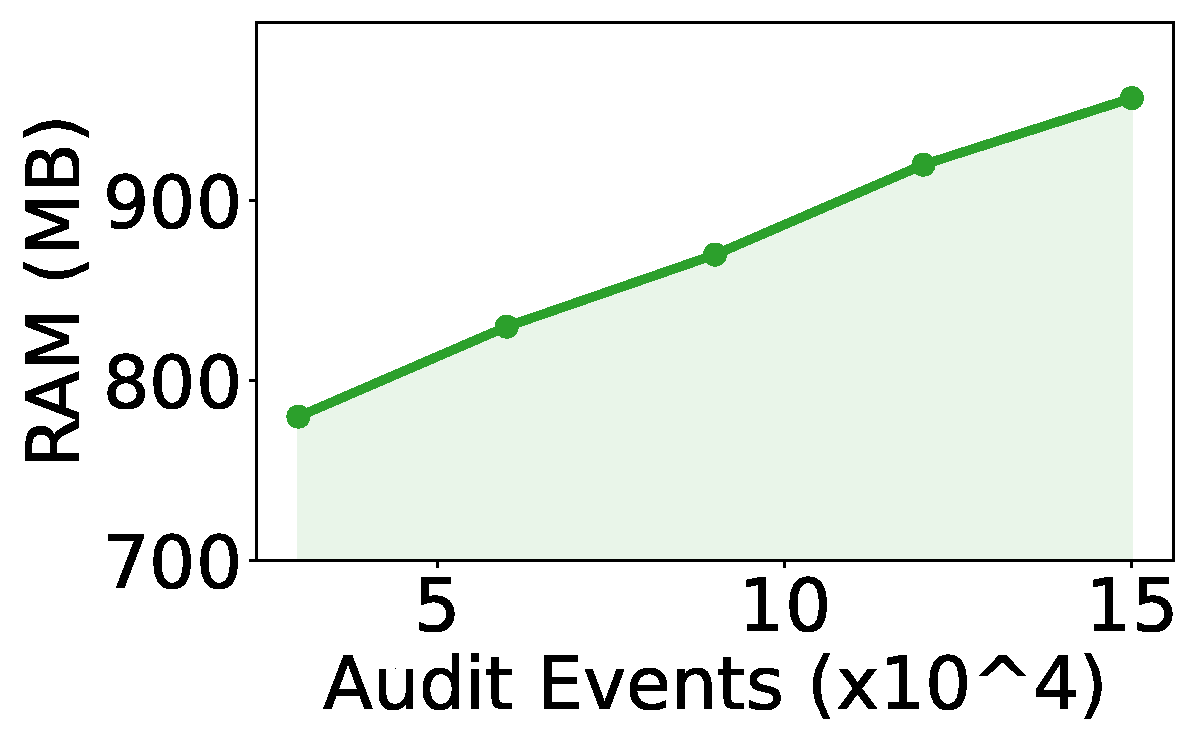
\includegraphics[width=0.50\textwidth]{fig/ram.pdf}
  \caption{RAM usage}
  \label{ram}
  \vspace{-2ex}
\end{figure}

\begin{figure}[t!]
  \centering
  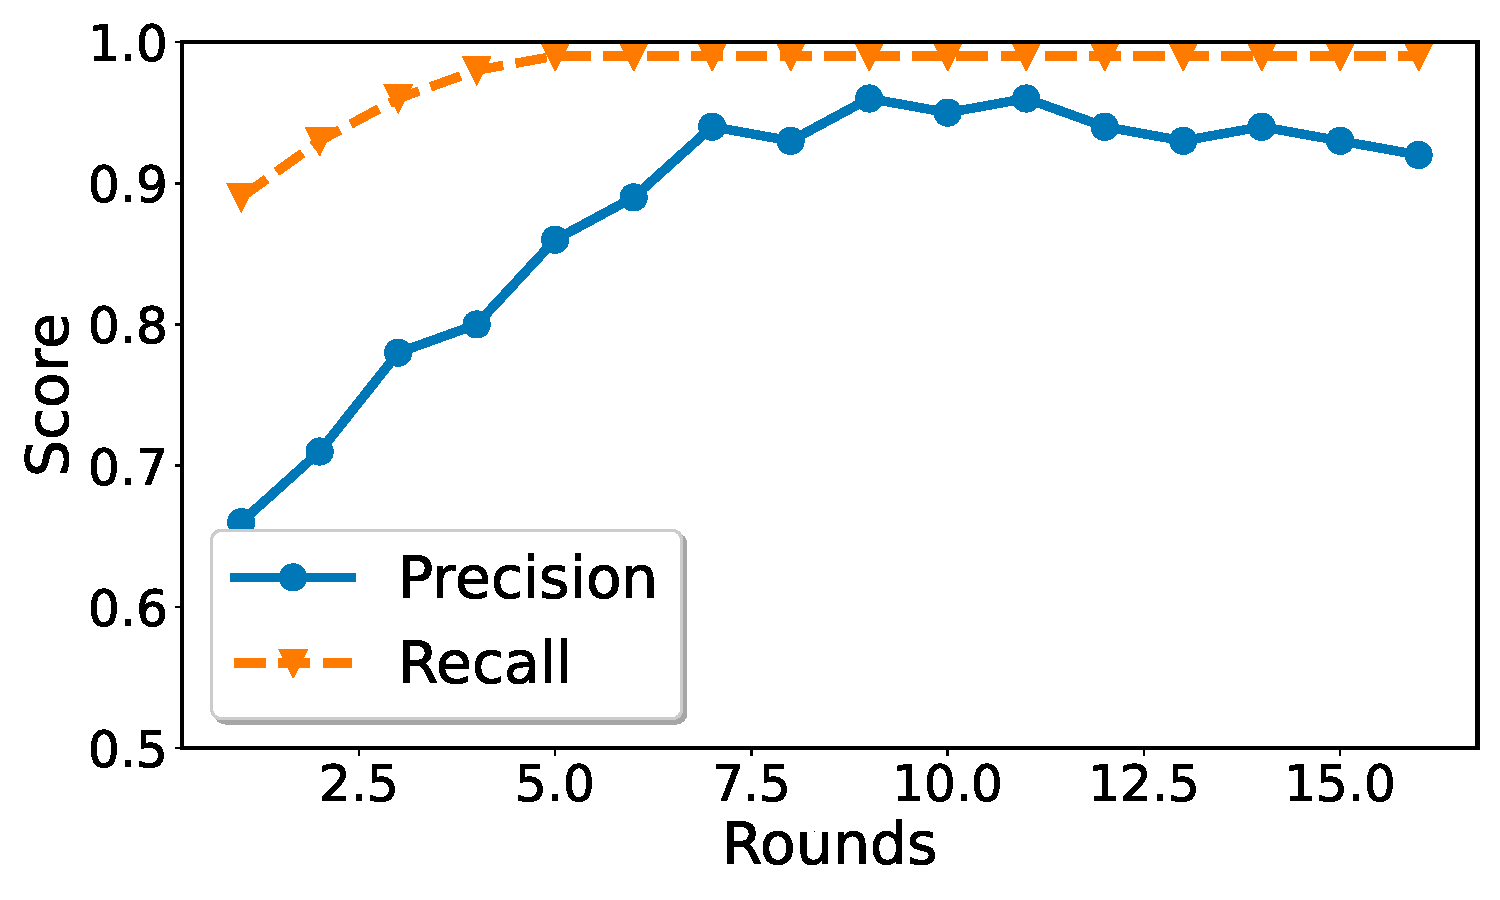
\includegraphics[width=0.50\textwidth]{fig/roundsvsscore.pdf}
  \caption{Federated Averaging Rounds vs Detection Performance.}
  \label{roundsvsscore}
  \vspace{-2ex}
\end{figure}

\begin{figure}[t!]
  \centering
  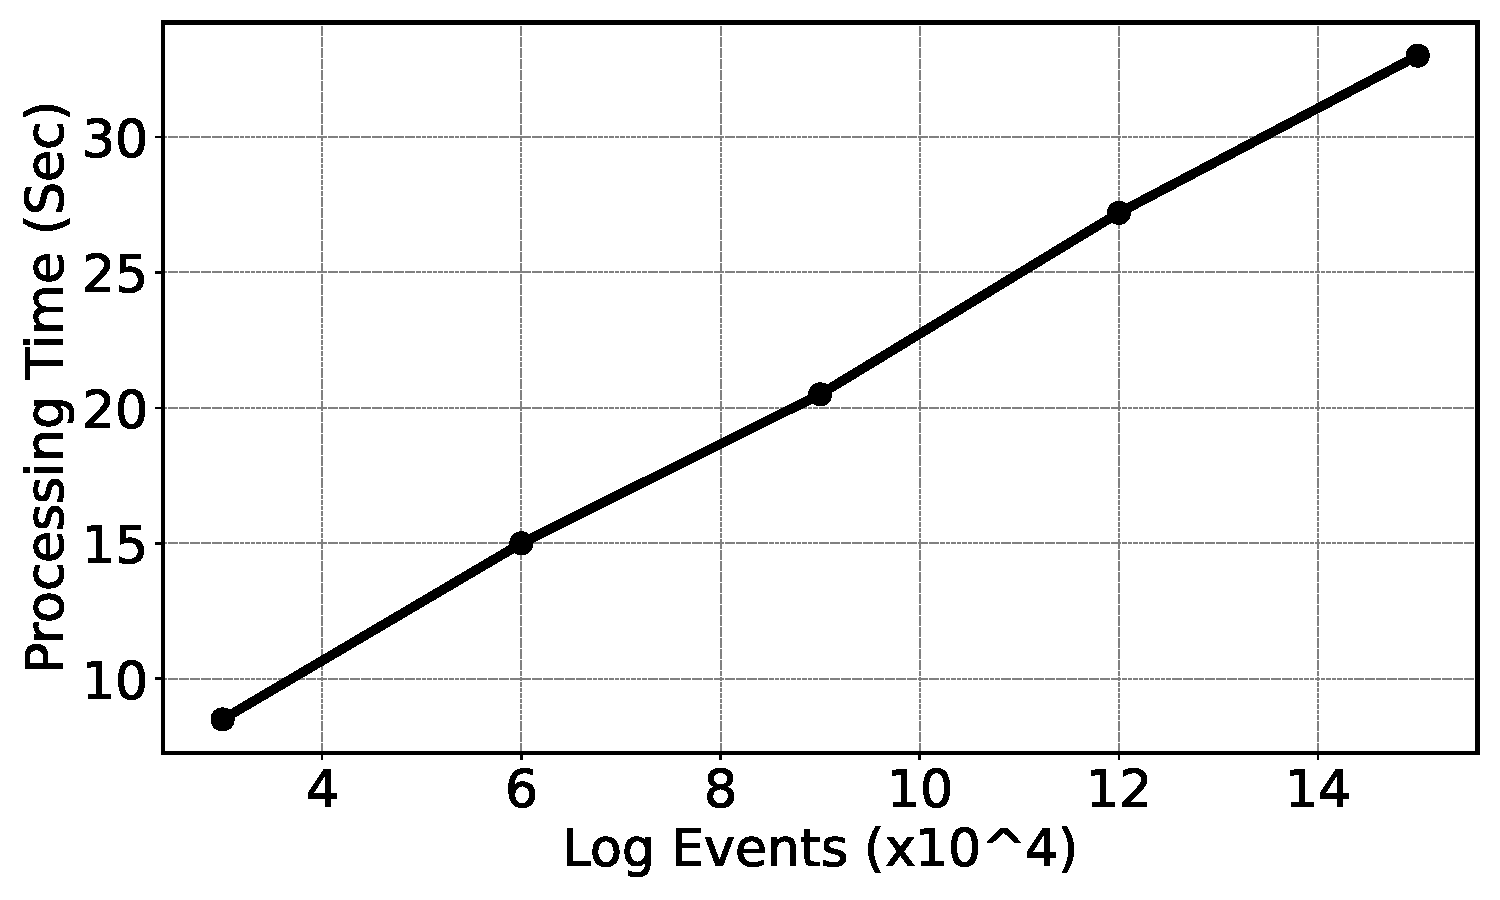
\includegraphics[width=0.50\textwidth]{fig/sizevstime.pdf}
  \caption{Processing Time for various Audit Event Sizes}
  \label{sizevstime}
  \vspace{-2ex}
\end{figure}

\begin{figure}[t!]
  \centering
  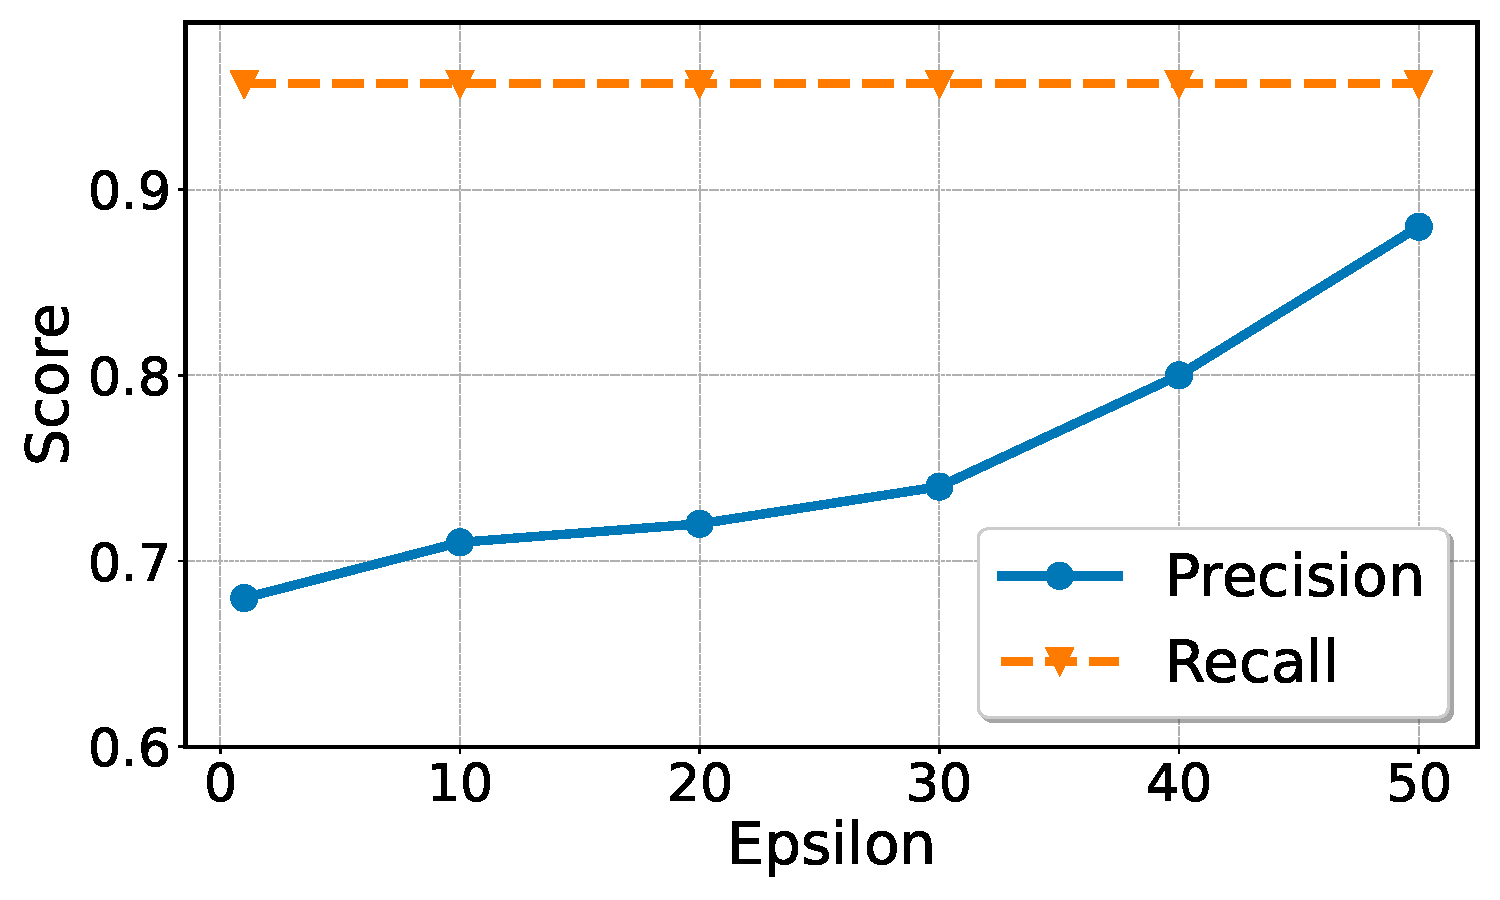
\includegraphics[width=0.50\textwidth]{fig/epsvsscore.pdf}
  \caption{Effect of Different LDP Noise Level on Detection Performance.}
  \label{epsvsscore}
  \vspace{-2ex}
\end{figure}

